%-------------------------------------------------------------------------------------------------%
% A related work section in which the relevant literature is presented and 
% linked to the project. 
% It should show that you clearly know the problem you plan to solve, 
% and that you master the related work. 

\chapter{Background \& Related work}
\label{chap:related}

\begin{figure}
  \centering
  \graphicspath{ {../../assets/diagrams/} }
  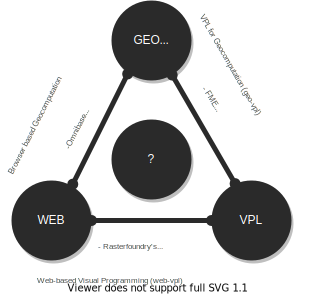
\includegraphics[width=250px]{geo-web-vpl.png}
  \caption{Triangle Model}
  \label{fig:triangle-model}
\end{figure}

This chapter offers an overview of the theoretical background that this study builds upon, alongside a review of related studies.
The study takes place at the intersection of three fields, represented by the corners of \reffig{fig:triangle-model}:
\begin{enumerate}[-]
  \item \refsec{sec:background-geo} covers the background on geocomputation
  \item \refsec{sec:background-web} covers the background on Web applications
  \item \refsec{sec:background-vpl} covers the background on Visual Programming Languages
\end{enumerate}

Additionally, while no project or study exist at the intersection of all three of these fields, we do find related studies which intersect two of these fields, represented by the edges of \reffig{fig:triangle-model}:
\begin{enumerate}[-]
  \item \refsec{sec:related-geoweb} reviews related works on browser-based geoprocessing
  \item \refsec{sec:related-geovpl} reviews related works on VPLs used for geo-computation
  \item \refsec{sec:related-webvpl} reviews related works on VPL web applications
\end{enumerate}

\section{Geocomputation}
\label{sec:background-geo}

This section offers a brief background on the wide topic of geocomputation. 

% PURPOSE: Show that you understand geo-computation | Show why the rest of the study will focus on the computer graphics side of things

Geocomputation is a central component of the wider field of geo-informatics. 
The term geocomputation, or geodata processing, is used to represent all types of computations performed on geographical data. 
Anything from the calculation of an area of a polygon, to \ac{crs} transformations, feature overlay, or converting a raster dataset into a vectorized dataset, is regarded as geocomputation.

It must be emphasized that a geocomputational procedure is always fully defined by and dependent upon its input and output data types (similar to any type of computation). 
This is also why geocomputation is seldom a \emph{goal} in itself, but much rather the \emph{means} to discovering geo-information. 

\begin{note}
  TODO: show images of geo-computation
\end{note}

\subsection{Similarities and differences with neighboring fields}

\begin{figure}
  \centering
  \graphicspath{ {../../assets/diagrams/} }
  \includegraphics[width=380px]{geocomputation.png}
  \caption{Geocomputation in relation to other fields}
  \label{fig:geocomputation}
\end{figure}

Geocomputation can be seen as an applied field of the more general field of computer graphics. 
Other applications of computer graphics include computer aided design (CAD), Building Information Modelling (BIM), molecular biology, medical imaging, robotics, but also special effects, video games, and graphic design.
For this reason, these applied fields can be regarded as neighbors to geocomputation \& GIS. 

It is important to recognize that certain geocomputational procedures fully overlap with computer graphics and these neighboring fields, while others are very specific to the field of GIS and geo-informatics.
As an example, matrix transformations and reprojections are commonplace in the wider field of computer graphics, but transformations formalized and structured in the form of \ac*{crs} is very specific to the field of GIS (See \reffig{fig:geocomputation}).
As such, geocomputational procedures can roughly be categorized in two fields: 
\begin{itemize}[-]
  \item geocomputations \emph{specific} to \ac{gis},
  \item \emph{common} computational geometry procedures
\end{itemize}
This categorization can be identified by noting if an operation appears in a neighboring field, or just in the field of \ac{gis}.

This \emph{specific} category exists because of \ac{gis}s foundation in the field of Geodesy, and the nature of geographical data. 
Geodata differentiates itself from any form of data by its sizable nature, and geospatial nature. 
GIS dataset sizes easily scale into terabytes of data, and each datum specifically represent a real, measured, earthly phenomenon.
This makes storage and accuracy much more relevant than other computer graphics applications. 

% NOTE TO SELF: GIVE CATEGORIES OF GEOCOMPUTATION IF IT IS ASKED FOR, OTHERWISE, LEAVE IT
% \subsection{Categories of Geocomputation}

% Geocomputation is a very broadly defined phenomenon, used to represent a great variety of computations. 
% To give an overview of this variety, a hierarchical subdivision of different types of geocomputation can be given, based on a subdivision of geodata types.

% The following distinctions are made between different geodata types:
% \begin{itemize}
%   \item Uniform
%   \subitem Rasters (Imagery)
%   \subitem Hexagons
%   \item Irregular, Vector-based
%   \subitem TIN 
%   \subitem solids
%   \subitem 3D Tiles
%   \item Semantic geodata:
%   \subitem Tabular geodata (QGIS)
%   \subitem Hierarchical, 'object oriented' geodata (GML / JSON) 
%   \item Point-cloud
% \end{itemize}

% Corresponding geocomputations are typically grouped together with one of these types of data. 
% However, this taxonomy is not perfect, since many computations exist \emph{between} between two different types of geodata.

% \subsubsection{Raster Geocomputation}

% - image processing
% - transformation kernels 

% \subsubsection{Vector Geocomputation}


% \subsubsection{Semantic Geocomputation}
% \begin{enumerate}[-]
%   \item often raster or vector at the core, with semantics layered on top 
% \end{enumerate}

% - 
% - 

% \subsubsection{Pointcloud Geocomputation}

\subsection{Geocomputation libraries}

\begin{figure}
  \centering
  \graphicspath{ {../../assets/images/background} }
  \includegraphics[width=380px]{all-geo-libraries-explained.jpg}
  \caption{Dependency graph of common geocomputation libraries. (This needs validation) }
  \label{fig:geolib-dependencies}
\end{figure}

Numerous geocomputational software libraries exist, written in a plethora of programming languages. 
Still, a certain 'Canon' can be defined based on popularity in terms of numbers of downloads, numbers of contributors, and number of dependent projects.  

Out of all open-source geocomputational libraries, the ones developed and maintained by the \ac{osgeo} (Source) can be regarded as the most significant to the field of \ac{gis}. 
These libraries include:
\begin{itemize}[]
  \item The \ac{gdal} (Source) 
  \item The Cartographic Projections and Coordinate Transformations Library titled PROJ (Source)
  \item The Geometry Engine Open Source (GEOS) (Source)
\end{itemize}
The geocomputations found in these libraries operate primarily on 2D / 2.5D raster and Simple Feature datasets (Source).
How these projects related together is presented by \reffig{fig:geolib-dependencies}.
Together, these libraries represent the core computational needs specific to the field of \ac{gis}. 

For the more 'common' computational geometry needs, the \ac{cgal} library is also widely used.

\section{Frontend web applications}
\label{sec:background-web}

This section offers a background on frontend web applications, their usage within the field of GIS, and developments in frontend web software development and frontend web technologies.

\begin{note}
  WHAT AM I GOING TO WRITE HERE: 
  - Build a base for all the times I will be speaking about web applications
  - Explain the typical structure, typical ingredients (HTML, CSS, JS) and the typical client-server architecture.
  Websites.
  - Then explain the client-heavy web-applications 
  - Then explain 
\end{note}

\subsection{Terminology}
In software development, the following dichotomies exist: 
\begin{enumerate}[-]
  \item Client and Server 
  \item Frontend and backend
  \item Native application, web application, and website
\end{enumerate}
While these dichotomies do overlap to an extend, years of interchangeable usage have lead to their differences often being overlooked. 
This study wishes to shed light on the relationships between these phenomena, as it will be essential in understanding its contribution.

\subsubsection*{Client and server}

\begin{figure}
  \centering
  \graphicspath{ {../../assets/images/misc/} }
  \includegraphics[width=380px]{todo.jpg}
  \caption{A typical client-server interaction) }
  \label{fig:client-server}
\end{figure}

First, the client-server model. 
The client-server model refers to a distributed application architecture which balances storage and processing responsibilities between two cooperating types of programs: 
Clients and servers.
In this model, a client sends a request to a server, and the server provides the response asked for (see \reffig{fig:client-server}).
While this model immediately invokes images of web clients and web servers, it is important to recognize that the client-server model is far older than either web applications, or the World Wide Web in general. 
It is an abstract computational model, of which the World Wide Web is just one example.
A corresponding client and server may even exist on the same machine. 

A program running on a machine can act as a client, a server, or both, based on the role this program sets out to fulfill in relationship to other programs. 
In this context, we make a distinction between \emph{Programs}, which refer to individual processes on either the side of the client or the server, and an \emph{application}, which represents the whole of corresponding client and server programs. 
If a client program runs without an active corresponding server it relies upon, we can say that the client \emph{program} functions, but the entire \emph{application} does not function. 

The client-server model is beneficial for sharing resources, both in terms of storage and processing. 
A distinction is made between centralized models, in which the bulk of these resources are centralized on one or more servers, and decentralized models, which distribute and offload some or all of the computational resources to the clients. 
A centralized model has the advantage of making clients simple and interchangeable, at the cost of making them highly reliant on the uptake of and connection to the server. This also generates more client-server traffic. 
A decentralized model makes clients independent and decreases traffic, at the cost of the complications caused by decentralized architectures. 
The choice between a centralized or decentralized client-server model is therefore highly reliant on the resources of client and server hardware, as well as the quality of the connection between the server and client.  

\subsubsection*{Frontend and backend}
The terms frontend and backend, though closely related to clients and servers, refer to different phenomenon. 
Both are separations of concerns, a design principle prevalent in computer science to specialize a program into separate responsibilities. 
However, client and server programs are defined by their separation into "requester" and "responder" roles, whereas the frontend and backend are defined by their separation into "presentation" and "data access" functions. 
Presentation functions are responsible for interacting with the end-user of the application, and is concerned with aspects such as user interface, user interaction, and rendering.
"data access" interacts with the physical hardware of the machine, and is concerned with aspects such as storage methods, database management, and scalability.  
It just so happens that the presentation functions often corresponds with a requester role,
and that data access functions often corresponds with the responder role.
However, this is never a given. 
A server can be responsible for providing both the frontend and backend functionality, in the case the presentation of an application is rendered on this server. 
This last sentence also sheds light on how server and client often correspond to the physical location of a program, whereas frontend and backend often refer to the functionality of a program.    

\subsubsection*{Native application, web application, and website}
Lastly, the differences between a web application, a website, and a native application. 

A native application is considered


% Nothing wrong with this chapter I think. Everything is there for a reason

% the latest in a series of geoprocessing attempts 
% we want to know what happened the previous times, so we will not try things that have already been tried before.

As a side note, client-side geocomputation is not to be confused with native geocomputation clients, which would include applications like QGIS \cite{qgis_community_qgis_2022}or ArcGIS \cite{esri_arcgis_2022}.
To circumvent this ambiguity, this study refers to client-side geocomputation as 'browser-based geocomputation'.



Web applications have specific advantages and disadvantages compared to native applications. 
The big advantages are that web applications are cross-platform by nature, and offers ease of accessibility, since no installment or app-store interaction is required to run or update the app. (src: vpl 2019, src: hybrid)
As soon as it can be found, it can be used.
The ability to share a full application with a link, or to embed it within the larger context of a webpage is also not trivial.
This changed with the introduction of the World Wide Web, and the web browser. 



Frontend, backend, client, server. 
None of these 

Now the most confusing part. 

The difference between a native application and a web application is, you guessed it, the web. A web application needs to be embedded within a browser in order to function. 

The term 'Web application' 
A web application, or "web app", is a type of distributed application software which runs exclusively in a web browser. 
In order to use a web application, it needs to be \emph{served} to the user by means of a web server. 

can refer to the client part, the server part, or the whole. 

This is in contrast to \emph{native} applications, which are 



Client-side
Server-side


% As the web and web technologies matures, new ways of using these technologies are discovered.

Since 2012, a trend of rich web-clients can be recognized \cite{hamilton_client-side_2014, panidi_hybrid_2015, kulawiak_analysis_2019}.
Browser clients had become powerful enough to allow for decentralized client-server models
This has led to single page application and client-side rendering, facilitated by 
However, the real facilitator of these developments are the browsers.
Improvements of the javascript runtime




The papers all speak of an emergent trend of thick-client web applications. 
Proponents of this trend argue that for certain applications, end users can benefit from dynamic, interactive websites which can immediately respond to a users input, rather than waiting on server round-trips necessary on static web-pages. 
And, by still being a webpage rather than a native application, users can access these applications without installment. 
The trend is made possible because of hardware improvements of client devices, as well as software improvements, like HTML5.

- quickly mention progessive web applications


To circumvent the 

browser-based applications

instead of other things like single page application, serverless appliations, or anything else. 


\begin{note}

  Sources: 

  (https://en.wikipedia.org/wiki/Web_application, i know i know, bad source, but this is more 'conventional wisdom' than true 'knowledge', couldnt find a more credible source, of what would make a person credible on this content)
  
  (https://en.wikipedia.org/wiki/Frontend_and_backend)
\end{note}

\subsection{WebAssembly}
\label{sec:background-wasm}

From all browser-based features, WebAssembly turned out to be a deciding factor of this study. This requires us to be aware of the state of WebAssembly and its performance considerations.

\ac{wasm} is officially dubbed the fourth type of programming language supported by all major web browsers, next to HTML, CSS, and JavaScript.
Strictly speaking however, WebAssembly not a language, but a binary instruction format for a stack-based virtual machine.
(SOURCE: https://webassembly.org/)
it can be used to, theoretically, run any application or library in a web browser, regardless of the language used to create it, be it C/C++, Python, C\#, Java, or Rust. 
This means that in order to create a web application, developers can now develop a normal, native application instead, which can then be compiled to WebAssembly, and served on the web just like any other web application. 
In this sense it offers a complete reverse workflow compared to the Electron based applications described above.  
If the line between web application and native application was already starting to get blurry, WebAssembly makes this line almost invisible. 

\subsubsection*{Limitations}

\emph{Almost} invisible, since there are quite a few caveats to the format. 
While in theory any application can be compiled to WebAssembly, in practice, not all applications turn into functional webassembly applications, due to certain factors.
These limitations can be split up into two groups: 
Limitations due to the web platform, and limitations due to the current state of the language and its host.

First of all, WebAssembly is required to adhere to the same containerization principles as javascript and the web at large. 
It cannot ask for resources which could be a potential security risk. 
As a consequence, any type of \ac{os} interaction such as opening a window, interacting with the file system, or drawing directly to the screen buffer, is off-limits.  

Secondly, WebAssembly is in its early phases as a language, and is intended as a simple, barebones, low-level compile target. 

currently does not support multithreading 
The abilities 

THIS ALL LEADS TO BOILERPLATE

There is also the concern that as of right now, a layer of javascript 'boilerplate' or 'glue code' is needed for many interactions between the user, the browser, and webassembly. 
For example, \ac{wasm} code is not able to directly manipulate DOM elements without calling javascript. 


\subsubsection{Background}

The original paper on WebAssembly was published on June 14, 2017 \cite{haas_bringing_2017}. The authors write that the reason behind the creation of WebAssembly is the observation that certain web applications started using JavaScript as a compile target, using a high-performance subset of JavaScript called 'asm.js' \cite{mozilla_asmjs_2013}. However, JavaScript remains a high-level, highly abstract programming language, which never intended to be used as a compile target. The discrepancy between intended use and actual use led to many complications for developers using JavaScript this way, but also for the developers of JavaScript itself \cite{haas_bringing_2017}. 
In order to relieve javascript of the responsibility of being a 'low-level' compilation target, developers of the four major browser vendors Mozilla, Google, Apple and Microsoft created WebAssembly and its corresponding paper, in a joined effort.

% This paper starts by promising WebAssembly as a save, fast, portable and compact compilation target. It continues by showing how previous attempts at low-level code on the web fail in at least one of these criteria, and that WebAssembly is the first to deliver on all of them. The follow up chapters cover a proof of memory safety, a proof of soundness of the language design, and the design decisions which had to be made to live up to those four criteria. These details will become relevant to the proposed thesis when reasoning about why WebAssembly might be faster in one case versus another.

\subsubsection*{Performance}

The initial performance benchmarks look promising. The majority of performance comparisons show that WebAssembly only takes 10\% longer than the native binary it was compared to \cite{haas_bringing_2017}. A later study confirms this by reproducing these benchmarks \cite{jangda_not_2019}. It even notices that improvements have been made in the two years between the studies. However, Jangda et. al. criticize the methodology of these benchmarks, stating that only small scale, scientific operations where benchmarked, each containing only 100 lines of code. The paper then continues to show WebAssembly is much more inefficient and inconsistent when it comes to larger applications which use IO operations and contain less-optimized code. These applications turn out to be up to twice as slow compared to native, according to their own, custom benchmarks. 
Jangda et. al. reason that some of this performance difference will disappear the more mature and adopted WebAssembly becomes, but state that WebAssembly has some unavoidable performance penalties as well. 
One of these penalties is the extra translation step, shown in reffig fig:wasm-trajectory, which is indeed unavoidable when utilizing an in-between compilation target. 

% Some studies have taken place evaluating \ac{wasm}'s performance for geospatial operations specifically. Melch performed extensive benchmarks on polygon simplification algorithms written in both javascript and WebAssembly \cite{melch_performance_2019}. It concludes by showing WebAssembly was not always faster, but considerably more consistent. Melch had this to say: "To call the WebAssembly code the coordinates will first have to be stored in a linear memory object. With short run times this overhead can exceed the performance gain through WebAssembly. The pure algorithm run time was always shorter with WebAssembly.". These findings match \cite{jangda_not_2019}, showing that sometimes the javascript JIT compilers of especially the chromium implementation outperform WebAssembly.

% Lastly, the sparse matrix research of Sandhu et al. will be mentioned. \cite{sandhu_sparse_2018}. It shows again that WebAssembly's performance gain is most notable when performing scientific computations. it states: "For JavaScript, we observed that the best performing browser demonstrated a slowdown of only 2.2x to 5.8x versus C. Somewhat surprisingly, for WebAssembly, we observed similar or better performance as compared to C, for the best performing browser.". It also shows how certain preconceptions must be disregarded during research. For example, it turned out that for WebAssembly and JavaScript, double-precision arithmetic was more performant than single-precision.

% A recent study concerned with watershed delineation \cite{sit_optimized_2019} also concluded client-side WebAssembly to be more performant than server-side C, which, as a side effect, enabled their application to be published on the web. 


Even though this proposed study falls in the category of scientific computation, these performance considerations will still have to be taken into account. The most important conclusion to to take away from prior research on WebAssembly is that \ac{wasm} must not be regarded as a 'drop-in replacement', as \cite{melch_performance_2019} puts it. Just like any language, WebAssembly has strengths and weaknesses. While \ac{wasm} is designed to be as unassumptious and unopinionated about its source language as possible, the implementations of host environments do favor certain programming patterns and data structures over others, and this will have to be taken into account when using the compile target.

\begin{figure}[!tbp]
  \centering
  \begin{minipage}[b]{0.80\textwidth}
    \graphicspath{ {../../assets/images/misc/} }
    \includegraphics[width=300px]{todo.jpg}
    \caption{Comparison of compilation trajectories}
    % based on the finding of \cite{jangda_not_2019}
    \label{fig:wasm-trajectory}
  \end{minipage}
\end{figure}

% \subsubsection*{Adoption \& Implementation}

% not in a vaccuum

% On 5 December 2019, the \ac{w3c} officially pronounced WebAssembly as the fourth programming language of the web \cite{w3c_world_2019}. Philippe Le Hégaret, the \ac{w3c} Project Lead, writes “The arrival of WebAssembly expands the range of applications that can be achieved by simply using Open Web Platform technologies. In a world where machine learning and Artificial Intelligence become more and more common, it is important to enable high performance applications on the Web, without compromising the safety of the users,”. Since then, most major browsers have added official WebAssembly support.

% As of writing this proposal, WebAssembly has of yet not seen widespread adoption in web developer communities. Opinions deviate, but in general, WebAssembly is considered a niche technology, often being named as 'experimental' and 'bleeding edge'. 

% This would explain why, to the best of the author's knowledge, not many projects and papers explicitly link WebAssembly and GIS. Papers on \ac{wasm} do state \textit{"3d data transformations and visualization"} as some of the examples of a high performance web applications \cite{haas_bringing_2017, jangda_not_2019}. What's more, certain GIS applications, like Google Earth, have started to use WebAssembly, as seen in \reffig{fig:google-earth} \cite{google_google_2020}. How it is used is unknown due to the engine being closed-source, but it is speculated that \ac{wasm} is used to access code written for the original C++-based desktop application.

% \begin{figure}[!tbp]
%   \centering
%   \begin{minipage}[b]{0.80\textwidth}
%     \includegraphics[width=\textwidth]{../images/google-earth-uses-webassembly.PNG}
%     \caption{Google Earth utilizing WebAssembly. Source: \cite{google_google_2020}}
%     \label{fig:google-earth}
%   \end{minipage}
% \end{figure}


% On the topic of WebAssembly, the most important conclusion to to take away from prior research is \ac{wasm} must not be regarded as a 'drop-in replacement', as \cite{melch_performance_2019} puts it. Just like any language, WebAssembly has strengths and weaknesses. While \ac{wasm} is designed to be as unassumptious and unopinionated about its source language as possible, the implementations of host environments do favor certain programming patterns and data structures over others, and this will have to be taken into account during the proposed study.

%%%%%%%%%%%%%%%%%%%%%%%%%%%%%%%%%%%%%%%%%%%%%%%%%%%%%%%%%%%%%%%%%%%%%%%%%%%%%%%

% Based on the studies on WebAssembly, we can conclude that the compilation peculiarities of WebAssembly have to be taken into account, as it cannot be regarded as a 'drop in replacement'. There is also a significant difference between using WebAssembly theoretically, and using it realistically. The studies on Client-side geoprocessing tell us that these implementation details can have vast consequences on user experience, and studies on the Geoweb express that this user experience is vital to FAIR, cross-community geoprocessing.

% What this means for the methodology, is that a significant portion of this study's attention will have to go to experimenting with different ways of compiling to WebAssembly, while making sure it can still be used in a realistic scenario.
% If it turns out that the use-case app can only be used by experienced end-users who take special \ac{wasm} considerations in mind, a big reason of using the web, namely its accessibility, would be lost.  


%%%%%%%%%%%%%%%%%%%%%%%%%%%%%%%%%%%%%%%%%%%%%%%%%%%%%%%%%%%%%%%%%%%%%%%%%%%%%%%
\subsubsection{(More on webassembly)}

Not just open source: process sharing using fully containerized instances. Think .

current vision / direction: containerized, sharable processes, together with web-based, front end visual programming environments ( RasterFoundry). Docker is usually named as a vision for these sharable processes.

\m{->} We do have examples of cloud-native geodata formats, and some examples of cloud-based geo-computation (RasterFoundry , Google Earth Engine, more). However, these approaches have not yet tried to use truly sharable, containerized geoprocesses using Docker or WebAssembly. 

\m{->} WebAssembly as a whole is underresearched. WebAssembly is not a fully virtualized container image, but just a binary set of instructions, meant to be executed on a virtual machine. Think of safe, cross-platform dll's. 
WebAssembly is in this regard more simple than docker, but this gives it more opportunities. 
WebAssembly runs in the browser for instance. 

\m{->} This opportunity to run in the browser would enable these cloud-native frontend environments to "dry-run" these processes from within the browser, completely detached from the server, as a means to experiment with processes on a small scale before applying them to a cloud native environment. 

\m{->} However, no implementations exist yet which combines containerized processes with these frontend computation environments. 

% # 2. BACKGROUND

% ## 2.1 The Web Browser & JavaScript
% -  main players (chrome, safari, firefox, edge(==chrome))
% - The browser js speed armsrace
% - How that lead to WebAssembly

% ## 2.2 The Geospatial Web. 
% [Still relevant]

% 2 biggest reasons against client-side geoprocessing: 
% - not performant enough
% - no equivalent to industry-standard libraries (CGAL / GDAL). 

% WebAssembly COULD solve both, so this study includes WebAssembly as 


% <br><br>

% .....

\section{Visual Programmming}
\label{sec:background-vpl}

%   \item Ladder Diagram (src), the industry-standard method of programming Programmable Logic Controllers (PLCs)

offers a rich background of prior research, and as such this literature review cannot be exhaustive. 
We instead focus on works which are particularly relevant to this studies' problem statement.

\begin{lstlisting} 
write something about : 
- cognitive_1996 
- advances_2004
- characterizing_2021

An increasing number of software applications are being written by end users 
without formal software development training. 
This inspired large technology companies such as Microsoft [91] and Amazon [90] 
to invest in low-code development environments empowering end users to 
create web and mobile applications. 
According to the 2019 Q1 Forrester report, the low-code market will witness an 
annual growth rate of 40\%, 
with spending forecast to reach \$21.2 billion by 2022 [102]. 
End-User Development (EUD) has emerged as a field that is concerned with 
tools and activities allowing end users 
who are not professional software developers to write software applications [11]. 
This is promising as end users know their own domain and needs more than anyone else, 
and are often aware of specificities in their respective contexts. 
Further, as end users outnumber developers with professional software development 
training by a factor of 30-to-1, 
EUD enables a much larger pool of people to participate in software development [12]. 
A visual programming language (VPL), among other EUD techniques, 
allows end users to create a program by piecing together graphical elements
 rather than textually specifying them [9]. 
Traditionally, visual programming has been successfully used to help novices
 learn basics of programming by visualizing elements of a program. 
However, visual programming is increasingly being used by end 
users in various domains to create and tailor applications that are useful 
beyond the realm of education. 
For instance, VPLs are now being used in fields such as 
the Internet of Things (IoT) [3], [10], mobile 
application development [51], robotics [8], and Virtual/Augmented Reality [4].
}

From characterizing_2021

other major use cases: 
- PLC: Ladder

\end{lstlisting}

\subsubsection*{Dataflow modelling}

\begin{lstlisting}
- Dataflow modelling is a field closely related to visual programming.
- However, where visual programming is concerned with many aspects, 
interface and usability being one of them, dataflow modelling is 
primairly concerned with the correct representation of data transformation.   
- within the field of dataflow modelling, it turned out that certain 
visual programming paradigms are advantageous, since they make parallel 
programming explicit. Thus, these fields are often named in conjunction. 
- The important take-away is that visual programming is not 
just a matter of UI or a stylistic choice.

- By more correctly representing dataflow and communicating 
opportunities for parallel computation, it can lead to faster applications.
\end{lstlisting}

\subsubsection*{REVIEW}
Challenges
\begin{lstlisting}
  - several challenges exist within the research field of visual programming. 
  - literature study (knowling what is and isnt being researched)
  - based upon : prior meta-analysis of 'characterizing_2021'
\end{lstlisting}

Difficulty in assessment of 'usability'
\begin{lstlisting}
  - usability is a nebulous phenomenon, hard to measure empirically.
  - no consensus on evaluation frameworks among VPL researchers. 

  BUT (leave this part, mention it later)
  - we will make no such attempt. usability serves as background motivation. 
  - this study assumes vpl's are 'in general' more usable to end-users 
  than text-based alternatives, based on the positive results of most of the 
  studies analysed by communicating_2021.   
\end{lstlisting}

web based visual programming is underresearched
\begin{lstlisting}
  
  large challenge
  - not many examples
    of these examples: 
    - no suitable starter projects
    - none are concerned with geometry

    - Visual programming environment for geo-computation 
    \emph{in a browser} has not been tried before. 


    "Finally, 53.3% (16) of the tools were available publicly with some documentation. 
    We strongly recommend that future tools are made available for end users as well as comprehensive documentation to ensure tool adoption and sustainability." communicating_2021 
   -> not fully related, but making this vpl web-based could seriously help this aspect of vpl assessment.   

\end{lstlisting}

VPL availabilty and life cycle
\begin{lstlisting}
Finally, (communicating_2021) names the 'life cycle' of apps created 
with the VPL as one of the most overlooked aspects within VPL research. 
- extend 
- debug
- publish
- run
\end{lstlisting}

%%%%%%%%%%%%%%%%%%%%%%%%%%%%%%%%%%%%%%%%%%%%%%%%%%%%%%%%%%%%%%%%%%%%%%%%%%%%%%%
%%%%%%%%%%%%%%%%%%%%%%%%%%%%%%%%%%%%%%%%%%%%%%%%%%%%%%%%%%%%%%%%%%%%%%%%%%%%%%%
%%%%%%%%%%%%%%%%%%%%%%%%%%%%%%%%%%%%%%%%%%%%%%%%%%%%%%%%%%%%%%%%%%%%%%%%%%%%%%%

\section{Browser-based geocomputation}
\label{sec:related-geoweb}

before we dive in, 

\subsection{The geospatial web}

Browser based geo-information systems have become an indispensable component of the wider geospatial software landscape. 
For the average person, an interactive \ac{gis} web application is often their first and only exposure to such a system, be it a web mapping service, a navigation system, or a pandemic outbreak dashboard. 

As stated in \refsec{sec:background-web}, web applications offer safety, distribution and accessibility advantages over native applications.

\subsection{Browser based geocomputation}

Despite the popularity of geographical web applications, the range of actual \ac{gis} abilities these applications are capable of is very limited. \ac{geocomputation} abilities, like CRS translations, bundle adjustment, interpolation or boolean operators, are usually not present within the same software environment as the web app. Consequently, current geospatial web applications serve for the most part as viewers; visualizers of pre-processed data. 

However, this limited range of capabilities inhibits the number of use cases geographical web applications can serve, and with that the usefulness of web \ac{gis} as a whole.
If web applications gain \ac{geocomputation} capabilities, they could grow to be just as diverse and useful as desktop \ac{gis} applications, with the added benefits of being a web application. It would allow for a new range of highly accessible and sharable geocomputation and analysis tools, which end-users could use to post-process and analyze geodata quickly, uniquely, and on demand.

... This is why browser-based geoprocessing is being researched ...

Browser-based geocomputation has seen some academic interest throughout the last decade \cite{hamilton_client-side_2014, panidi_hybrid_2015, kulawiak_analysis_2019}.

The aforementioned papers each try to apply this trend to the field of geo-informatics. 
Hamilton et. al. created a such a 'thick-client', capable of replacing certain elements of server-side geoprocessing \cite{hamilton_client-side_2014}. 
However, the results are unfavorable towards JavaScript. 
The paper states how "the current implementation of web browsers are limited in their ability to execute JavaScript geoprocessing and not yet prepared to process data sizes larger than about 7,000 to 10,000 vertices before either prompting an unresponsive script warning in the browser or potentially losing the interest of the user.". While these findings are insightful, they are not directly applicable to the efforts of this study proposal. Three reasons for this:

\begin{itemize}
  \item The paper stems from 2014. Since then, web browsers have seen a significant increase in performance thanks to advancements in JavaScript JIT compilers \cite{haas_bringing_2017, kulawiak_analysis_2019}. 
  \item The paper does not use compile-time optimizations. The authors could have utilized 'asm.js' \cite{mozilla_asmjs_2013} which did exist at the time. 
  \item The paper uses a javascript library which was never designed to handle large datasets.
\end{itemize}

The same statements can be made about similar efforts of Panidi et. al. \cite{panidi_hybrid_2015}. 
However, Panidi et. al. never proposed client-side geoprocessing as a replacement of server-side geoprocessing. Instead, the authors propose a hybrid approach, combining the advantages of server-side and client-side geoprocessing. 
They also present the observation that client-side versus server-side geoprocessing shouldn't necessarily be a compassion of performance. 
"User convenience" as they put it, might dictate the usage of client-side geoprocessing in certain situations, despite speed considerations \cite{panidi_hybrid_2015}. 

This concern the general web community would label as \ac{ux}, is shared by a more recent paper \cite{kulawiak_analysis_2019}. 
Their article examines the current state of the web from the point of view of developing cost-effective Web-GIS applications for companies and institutions. 
Their research reaches a conclusion favorable towards client-side data processing: "[Client-side data processing], in particular, shows new opportunities for cost optimization of Web-GIS development and deployment. 
The introduction of HTML5 has permitted for construction of platform-independent thick clients which offer data processing performance which under the right circumstances may be close to that of server-side solutions. 
In this context, institutions [...] should consider implementing Web-GIS with client-side data processing, which could result in cost savings without negative impacts on the user experience.".

% Based on the topic of client-side geospatial processing, we can state that web technologies contain a very dynamic temporal component. All research can become outdated, but performance analysis of web technologies are especially quick to change.  

From these papers we can conclude a true academic and even commercial interest in client-side geoprocessing in the last decade. However, researchers quickly encounter problems during practical implementations in the past. This might not hold up thanks to recent browser features, but these papers still show how small, practical implementation details can relate to considerable changes in \ac{ux}. 

Additionally, to the best of the authors's knowledge, all papers concerned with browser-based geoprocessing either tried to use existing JavaScript libraries, or tried to write their own WebAssembly / JavaScript libraries. No studies have been performed on the topic of compiling existing C++/Rust geoprocessing libraries to the web. 




%%%%%%%%%%%%%%%%%%%%%%%%%%%%%%%%%%%%%%%%%%%%%%%%%%%%%%%%%%%%%%%%%%%%%%%%%%%%%%%
\subsubsection*{Browser based geoprocessing software}

% https://www.azavea.com/blog/2016/09/26/raster-foundry-model-lab-phase-ii-sbir/
% https://geotiff.io/
- >
% https://www.eclipse.org/community/eclipse_newsletter/2018/december/geotrellis.php 
% -> ModelLab
% -> " Online tool to build, store, and execute complex geospatial models "
% - Mobius Modeller : https://mobius.design-automation.net/pages/mobius_modeller.html
% - GeoTIFF : https://app.geotiff.io/
These are all similar efforts, also hooked up to the OGC cloud native developments
Geofront will differ, for it focusses on 3D \& Point clouds instead of rasters \& map algebra, and focusses on client-side geodata consumption \& processing instead of being a server-side pipeline configurer.

ModelLab says this : "Widespread access to frequent, high-resolution Earth observation imagery has created the need for innovative tools like ModelLab that will help individuals and organizations to effectively access, analyze, edit, and visualize remotely sensed data in transformative new ways without years of specialized training or ongoing investments in proprietary software and technology infrastructure. "


%%%%%%%%%%%%%%%%%%%%%%%%%%%%%%%%%%%%%%%%%%%%%%%%%%%%%%%%%%%%%%%%%%%%%%%%%%%%%%%%
% - https://openscad.org/

%%%%%%%%%%%%%%%%%%%%%%%%%%%%%%%%%%%%%%%%%%%%%%%%%%%%%%%%%%%%%%%%%%%%%%%%%%%%%%%
\subsubsection*{Client-side geoprocessing}

% NEW PRACTICAL ATTEMPT. WHY? 
% - csg still has a lot of potential
% - previous studies:
%   - are dated
%   - prioritized theory over practicalities
%   - utilized the web's major feature of Accessibility and the clients feature of    
%     Interactivity inadequately 
%   - were not creative enough in terms of possible use-cases 

While these studies pose a strong theoretical case for client-side geoprocessing, their practical implementations were less convincing \todo{TODO: Figure out how to phrase this better}. 
The implementations of \cite{panidi_hybrid_2015, hamilton_client-side_2014} were written in a time before WebAssembly \& major javascript optimizations, and the study of \cite{kulawiak_analysis_2019} prioritized theory over practice. 


This study recognizes a need for a new, practical attempt at client-side geoprocessing. 
Client-side geoprocessing is a promising prospect with potentially many use cases.
Previous attempts are either dated due to the web's rapid advancements, or chose theory over practice.

In addition, the implementations lacked creativity \todo{This needs a better phrase, but it really is the most direct way of putting it}. 

The applications were either meant as small demo's, without a clear target audience or use-case in mind (just a way to demo performance), or as highly specified debugging tool for the authors.   
But, as mentioned before, a major advantage of Web applications over native applications is \emph{Accessibility}, and a major advantage of client-focussed web apps over server-focussed web apps is \emph{Interactivity}. 
By creating a client-side web application which is neither accessible nor interactive, the main incentive for creating a client-side web app is lost.
Additionally, by forgoing the question of accessibility, many auxiliary use-cases of client-side geoprocessing where overlooked.

%%%%%%%%%%%%%%%%%%%%%%%%%%%%%%%%%%%%%%%%%%%%%%%%%%%%%%%%%%%%%%%%%%%%%%%%%%%%%%%
%%%%%%%%%%%%%%%%%%%%%%%%%%%%%%%%%%%%%%%%%%%%%%%%%%%%%%%%%%%%%%%%%%%%%%%%%%%%%%%
%%%%%%%%%%%%%%%%%%%%%%%%%%%%%%%%%%%%%%%%%%%%%%%%%%%%%%%%%%%%%%%%%%%%%%%%%%%%%%%

\subsection*{The Cloud Native Geospatial movement}

( Not sure if I wanna go there... )

% Establish OGC in two sentences, mentioning their name and Vision
The Open Geospatial Consortium (OGC)...
Mission: FAIR Geodata 

% Establish Cloud Native movement.
% GIS as one big LAN party
A prominent development within the OGC is the recent effort towards a \textbf{"Cloud Native Geospatial"} future. 
This initiative aims to radically simplify geodata storehouses to static servers serving large, singular binary geodata files. All processing and analysis of this geodata can then be performed by separate cloud-based web services. 
This architecture has many advantages over current geodata storage and analysis methods:
\begin{itemize}
  \item These new Cloud Native geodata formats are much cheaper to access by front-end and back-end services, compared to active services.
  \item Substituting active SQL or noSQL databases by static binary files is easier and cheaper for data providers, leading to more and more readily available geodata.
  \item By using supercomputers (Microsoft Planetary Computer) and cloud-storage (AWS), Geodata processes could make use of near-infinite computational and storage resources. 
  \item By having all data centralized in one location or type of location, new, large scale patterns within our geodata could be discovered.  
  \item For web GIS, this would offer direct data streaming options, similar to services like "Netflix" or "Spotify".  
\end{itemize}

These features may have a far reaching impact on society. Chris Holmes, forerunner of the cloud-native geospatial movement, envisions what the movement could mean for even non-GIS users: 
\emph{
  With the introduction of accessible, centralized data, and the dramatically different workflows that follow, Cloud Native Geospatial has the potential to introduce new, non-specialized users to the power of geospatial information that GIS practitioners have enjoyed for decades. [...]. The ecosystem of geospatial experts will collaborate to create analyses and insight, but any non-expert user will be able to select and apply those to the geographic area they care about. \~ Chris Holmes
}
% This is also reflected by cloud-native based tools like (Google Earth Engine or RasterFoundry) may achieve such a feed, by being web based and stuff...
All these reasons explain why the OGC and many other parties are now actively pursuing this vision.

But while this vision is in active development, many large-scale challenges are still in its way. 
One of the most important challenges is the required paradigm shift within geo-computation / geoprocessing workflows. 
The current, common geo-computation workflow of retrieving online data, only to run it through a local process and send the resulting data back into servers, will have to be reversed: In a cloud-native future, we will not retrieve data for our local process, but we will upload our process to the data.  
This introduces a sizable challenge: \textbf{Portable, Containerized Geo-computation}.

% \textbf{and the algorithms powering the processing can be shared online and customized collaboratively}. -> Chris again

% \begin{itemize}
%   \item Up to this point, the world of GIS has done a considerable effort to make geodata more Findable, Accessible, Interoperable, and Reusable. The challenge of Portable geo-computation now forces us to extend the effort of FAIR geodata to FAIR geodata computation as well.  
%   \item If we want our geodata processes to be just as portable as the geodata it takes as input, then perhaps the FAIR paradigm should extend from FAIR geodata to FAIR geodata processing . FAIR geo-computation.
%   \item Furthermore, it remains a mystery how these containerized containerized processes will be configured and accessed by frontend computation environments. 
%   \item Holmes: one of the vital ingredients: \emph{"and the algorithms powering the processing can be shared online and customized collaboratively"}.
% \end{itemize}

The challenge of sharing and chaining together containerized fragments of geoprocesses to a variety of environments will require more than just open source collaboration. 
This study interprets the challenge of portable geo-computation by means of the FAIR paradigm. 
If geodata processes need to be just as portable as the geodata forming the input and output, then perhaps the FAIR paradigm should extend from FAIR geodata to FAIR geodata \emph{processing} as well.
The challenge facing the cloud-native vision then becomes: \textbf{How to make geo-computation Findable, Accessible, Interoperable, and Reusable?} 
This links back to containerization, for containerization is a very powerful method of making geo-computation more Interoperable and Reusable.

% state of the art regarding this issue, make a path towards the particular thesis, and why it is an application
The current state of the art is far removed from either portable or FAIR geo-computation. 
\todo{Improve this intro}
\begin{itemize}
  \item current methods: Docker, and some geo-computation platforms.
  \item Not many implementations using WebAssembly, while this is a prime candidate: Even the guy who made Docker said so. 
  \item ignore the cloud: focus on the act of containerizing geoprocesses using webassembly an sich
\end{itemize}

\section{Visual programming and geocomputation}
\label{sec:related-geovpl}

acknoledgements
- Name similar studies or things 
  - Ravi Peter: awesome c++ based application 
    - not web
    - not formal reseach

\begin{lstlisting}
  (explain the use-case of vpl's within the field of geo-informatics, 
  why they are significant to us) 
  within geomatics

  - data translation: FME 
  - cloud-native computation: modellab in rasterfoundry
    - link to dataflow modelling
  - debugging & experimentation: GeoFlow 
  
\end{lstlisting}


This advantage of interactive, low-code automation is why the VPL continues to be a popular interface within the field of GIS, as well as in neighboring fields like BIM, CAD, Shader Programming and Procedural Geometry. 
All these fields benefit from the combination of both low-code automation and visual debugging.
% The field of geo-informatics also appreciates the 'dataflow modelling' aspects (TODO FIX THIS SENTENCE)

Within the field of geo informatics, \ac{vpl}s are not a new phenomenon. VPLs have been used for decades to specify geodata transformations and performing spatial analyses.  
SaveSoft's FME (SOURCE) is a good example of this. This Extract Load Transform (ETL) platform automates data integration, and is widely used by GIS experts.



% The environment proposed by this thesis builds from Ravi Peter's work. GeoFront can be seen as GeoFlow, but in a web browser. However, the introduction of this web component significantly changes the purpose and use-case of GeoFront compared to GeoFlow. 

% GeoFlow's mission: Create a geoprocessing pipeline in a visual environment, in order to speed up and improve the quality of the development process of this pipeline "FOR YOURSELF", compared to text-based methods. This speed and quality comes from the fact that the visual environment makes rapid experimentation and evaluation possible. This is especially helpful for non-determinant processes, or processes containing 'magic' number parameters. Examples of these are RANSAC algorithms. 

% GeoFront's mission: Use the vpl to make rapid experimentation and evaluation of your geoprocessing functions possible FOR OTHERS. This enables others to rapidly utilize your geoprocessing method. The primary use case of this is collaboration: Rapidly publish ones results, demonstrate reproducibility, retrieve feedback, etc.   


% Visual programming environment for geo-computation (geo-vpl) has been tried before, natively ( Grasshopper , FME , GeoNodes , Blender Geometry Nodes ). 


% The entire application runs client-side in a browser, and uses a visual programming language as its primary \ac{gui}.
% The main goal and feature of geofront is to take existing low level geo-computation libraries, and to make these interactively usable on the web. 
% These libraries include a limited set of CGAL operations, complied from C++, and various geo-computation algorithms such as Startin, written in Rust. 
% Being a visual programming language, GeoFront can be used to interactively alter the geodata pipeline. 
% In between products can quickly be inspected using a 3D viewer.

% We test how well contemporary web technologies support such an application, as well as judge aspects such as accessibility \& performance of said application. We also judge if this type of application is indeed beneficial and usable as a scripting / demo environment.  

% These features could all be implemented by normal means ( buttons, panels, sliders ) -->

% Where ModelLab is build on top of recent improvements to the accessability of satellite imagery, GeoFront is build in anticipation to a similar development for point cloud datasets with the introduction of COPC.  The focus of Geofront is therefore on point cloud processing, and point-cloud based modelling, such as Digital Terrain Models (DTM). 


\subsubsection*{ In Neighboring fields }
In Geometry Computation \& Visualization:

\begin{lstlisting} 
   - Besides the use cases already mentioned, a significant number of 
   visual programming applications are emerging in fields concerned 
   with 2D and 3D geometry creation \& visualization. 

  PROCEDURAL GEOMETRY 
    - Rhino: Grasshopper
    - Revit: Dynamo  
    - Blender: Geometry Nodes
    - Houdini: Procedural Modelling
  
  TEXTURES AND SHADERS
    - Blender: Shader Nodes
    - Adobe: Substance Designer
    - Unreal Engine: Material Nodes
    - Unity: Shader Graph
    - Houdini: FX

  These are all popular applications, many users, multiple courses and tutorials, 

  The persistence of visual programming within the field of shaders and
  geometry, suggests that visual programming languages are advantageous in
  situations where a 'visual' product requires debugging during development. 
\end{lstlisting}


% -> testing & reproducability.
% RANSAC -> many 'magic' parameter. They need to be discovered by 'play'
% Jonathan blow -> using interactive applications, an intrinsic understanding can be gained without explicit communication.
% Game Of Life -> impossibility of 'proving' behaviour systems. 


\section{Browser-based visual programming}
\label{sec:related-webvpl}

The number of visual programming languages written as web applications is surprisingly low. 
Most applications are educational


(https://www.ucode.com/coding-classes-for-kids/is-scratch-the-same-as-blockly)

(https://developers.google.com/blockly/)

(https://developers.googleblog.com/2019/01/scratch-30s-new-programming-blocks.html)

% (SOURCE: https://dl.acm.org/doi/fullHtml/10.1145/1592761.1592779?casa_token=cJ1iX1YYimkAAAAA:YVyp3KFiKwD2GMuBUUIgvibbNsEgndqNQzehRnCosCpyEx51C_uNpi2D4-lsE-x88hQFSWcbTfrP_w)

Does exist, but very niche. 
best example is Scratch, an educational tool.
digging in github reaps some results, mostly experimental, in development applications

\section{Browser-based Visual programming and geocomputation} 
To the best of the author's knowledge, a publicly available visual programming language which is both able to run and execute in a browser, and is able to be used for geodata computation, does not exist. 
However, certain applications and studies come close. 
The best example of a similar application this study was able to find, is RasterFoundry's modellab application
Best example: rasterfoundry, modellab but doesnt really count, since cacluations are performed in the backend (as far as we know). 
Also, implementation details are not public. 


